\section{Specifica dei casi d'uso}
In questa sezione si analizzeranno le classi e come sono relazionate tra loro, daremo un'occhiata ai sequence diagram (in particolare quelli riguardanti due funzionalità dell'applicazione) e agli statechart relativi all'interfaccia grafica. Per fare ciò utilizzeremo:
\begin{enumerate}
  \item Class diagram.
  \item Sequence diagram.
  \item State chart
\end{enumerate}
\subsection{Classi, oggetti e relazioni di analisi}
In questa sezione utilizzeremo i \textit{class diagram} per farci un idea della relazione tra le classi, prima di tutto diamo uno sguardo alla struttura generale che abbiamo creato in fase di analisi:
\begin{figure}[H]
  \centering
  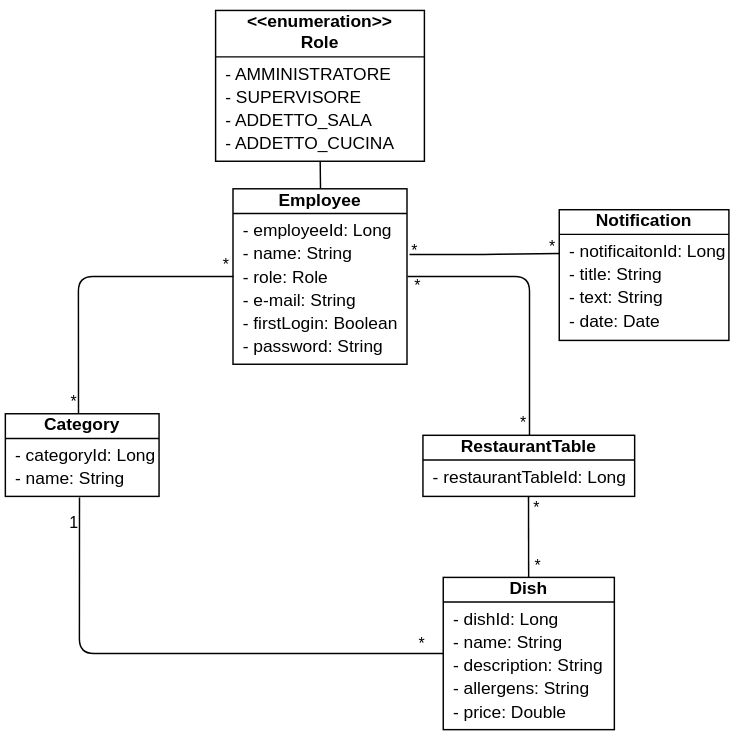
\includegraphics[scale=0.6]{img/class_diagrams/generalClassDiagram.png}
  \caption{Class diagram delle entità}
\end{figure}
D'ora in poi invece, i \textit{class diagram} mostrati, saranno quelli delle funzionalità che sono state assegnate al team di sviluppo.
\newpage
\subsection{Class diagram di analisi - Gestione menù}
In questo class diagram viene analizzato il punto 3 della traccia ovvero la gestione del menù.
\begin{figure}[H]
  \centering
  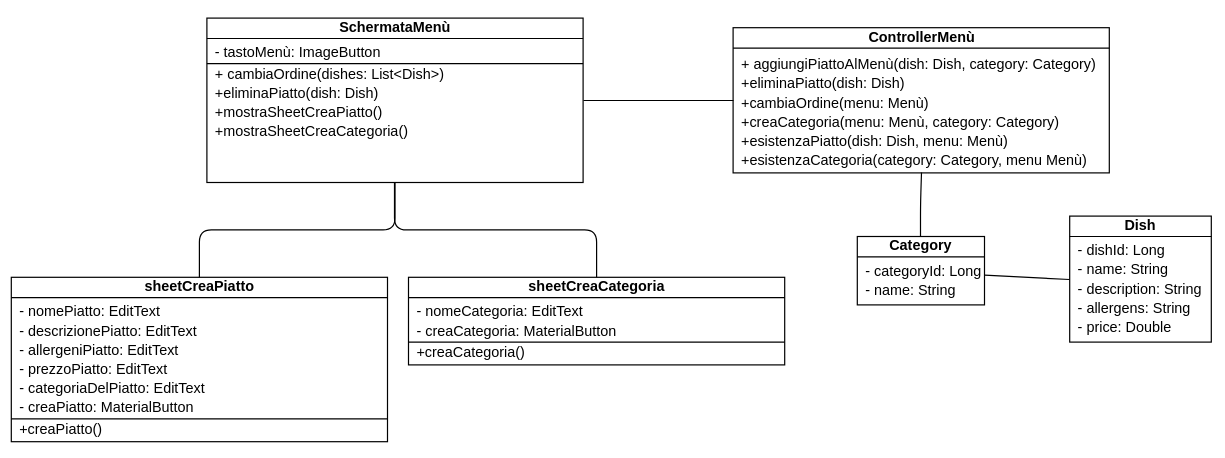
\includegraphics[scale=0.55]{img/class_diagrams/gestioneMenu_class_diagram.png}
  \caption{Class diagram della gestione del menù}
\end{figure}
\newpage
\subsubsection{Class diagram - Creazione utenza}
Nel seguente class diagram verrà analizzato il punto 1, quello nel quale si richiede la creazione di un utente e l'eventuale cambio password nel caso in cui si tratti del primo login, il cambio password verrà però affrontato in un \textit{class diagram} successivo, in modo da poter comprendere anche l'accesso alla piattaforma.

\begin{figure}[H]
  \centering
  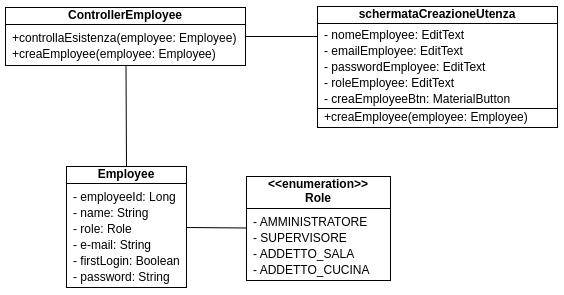
\includegraphics[scale=0.75]{img/class_diagrams/creazioneUtenza_class_diagram.png}
  \caption{Class diagram per la creazione utenze}
\end{figure}
\subsubsection{Class diagram - Accesso alla piattaforma}
Adesso, come detto in precedenza, analizzeremo l'accesso (con conseguente cambio password) alla piattaforma.
\begin{figure}[H]
  \centering
  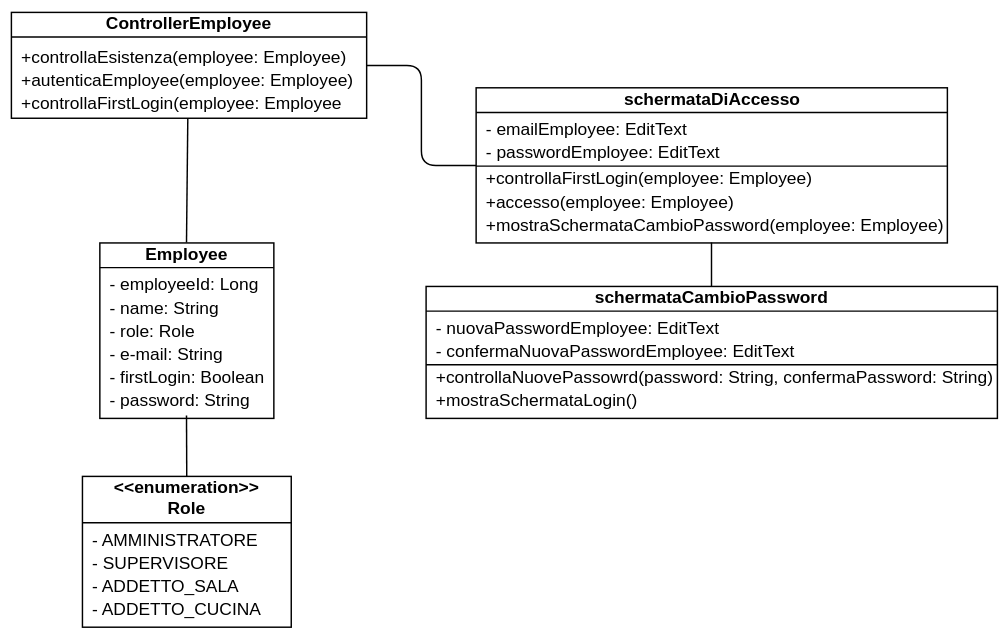
\includegraphics[scale=0.5]{img/class_diagrams/accessoCambioPassword_class_diagram.png}
  \caption{Class diagram dell'accesso alla piattaforma}
\end{figure}
\subsubsection{Class diagram - Gestione tavoli}
Il seguente \textit{class diagram} analizza il punto 6, quindi creazione ordinazioni indicando l'identificativo del tavolo e gli elementi del menù da aggiungere al tavolo.
\begin{figure}[H]
  \centering
  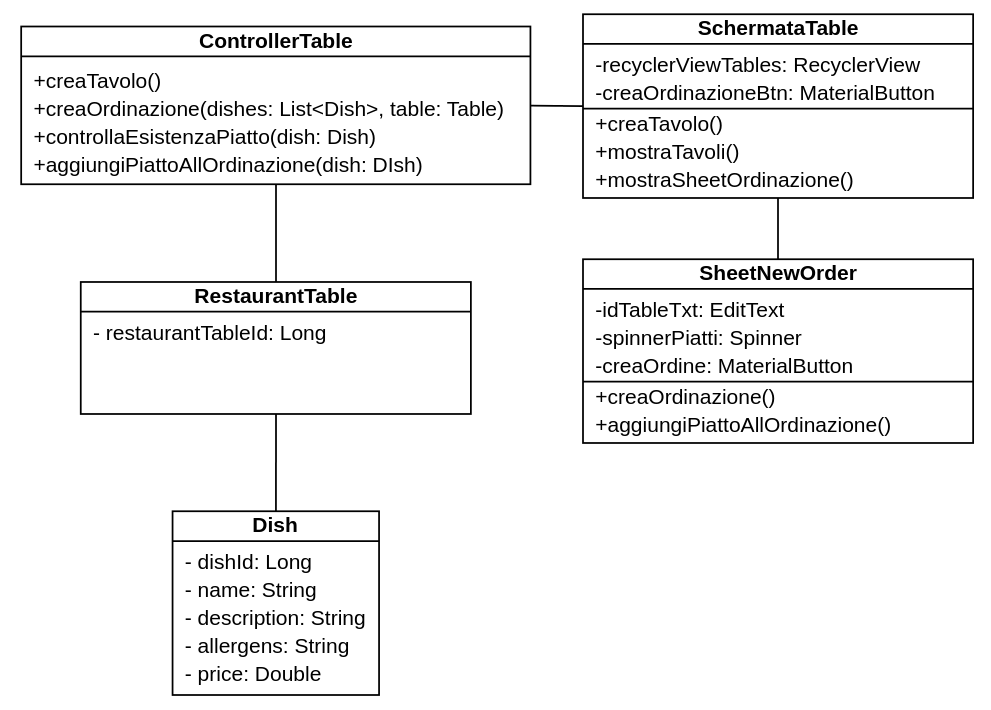
\includegraphics[scale=0.5]{img/class_diagrams/gestioneTavoli_class_diagram.png}
  \caption{Class diagram della gestione dei tavoli}
\end{figure}
\newpage
\subsubsection{Class diagram - Gestione notifiche}
Il seguente \textit{class diagram} analizza il punto 13, quindi creazione di avvisi (notifiche), al quale verrà aggiunta la visualizzazione delle notifiche.
\begin{figure}[H]
  \centering
  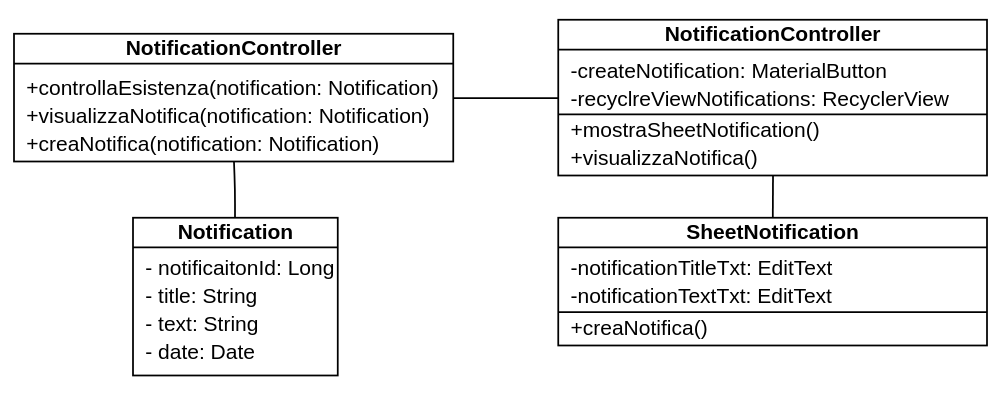
\includegraphics[scale=0.5]{img/class_diagrams/gestioneNotifiche_class_diagram.png}
  \caption{Class diagram della gestione delle notifiche}
\end{figure}
\newpage
\subsection{Sequence diagram}
In questa sezione verranno analizzati due casi d'uso ritenuti fondamentali per questo progetto, in particolare analizzeremo la \textbf{creazione di un piatto}, in quanto parte fondamentale per la gestione di un'attività di ristorazione e la \textbf{gestione delle notifiche}, quest'ultima è stata scelta poiché tutti i dipendenti possono ricevere e visualizzare notifiche ed è fondamentale ai fini del corretto svolgimento dell'attività.
\subsubsection{Sequence diagram - Creazione piatto}
In questo \textit{sequence diagram} l'attore è un superivsore o l'amministratore, sono gli unici due ruoli con i permessi per la creazione di un piatto. I controlli che verranno fatti saranno sull'esistenza della categoria selezionata, verrà controllato se il piatto è già presente ed eventualmente se uno o più campi sono vuoti o non validi.
\begin{figure}[H]
  \centering
  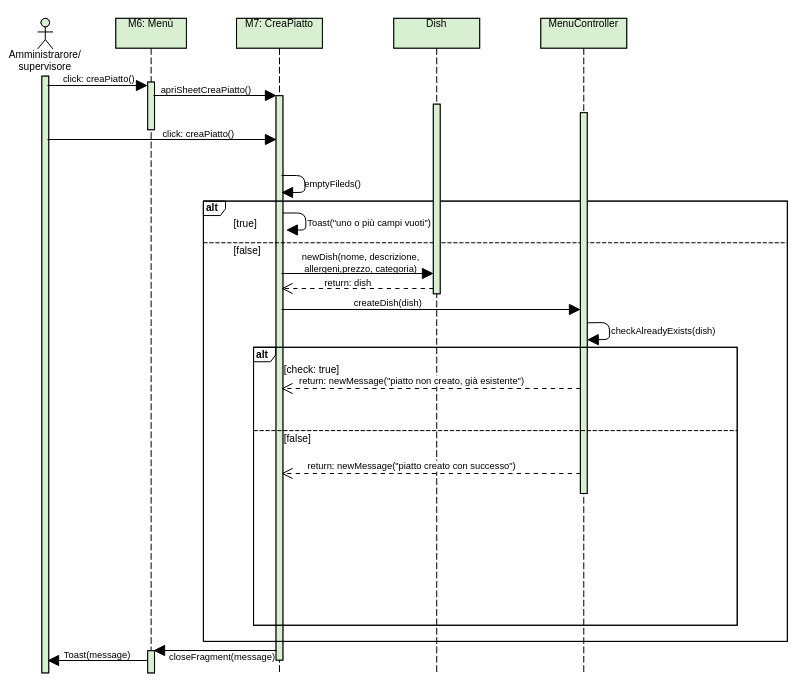
\includegraphics[scale=0.8]{img/sequence/creazionePiatto_sequence_diagram.png}
  \caption{Sequence diagram della creazione di un piatto}
\end{figure}

\subsubsection{Sequence diagram - Creazione piatto}
In questo \textit{sequence diagram} l'attore è un superivsore o l'amministratore, sono gli unici due ruoli con i permessi per la creazione di un piatto. I controlli che verranno fatti saranno sull'esistenza della categoria selezionata, verrà controllato se il piatto è già presente ed eventualmente se uno o più campi sono vuoti o non validi.
\begin{figure}[H]
  \centering
  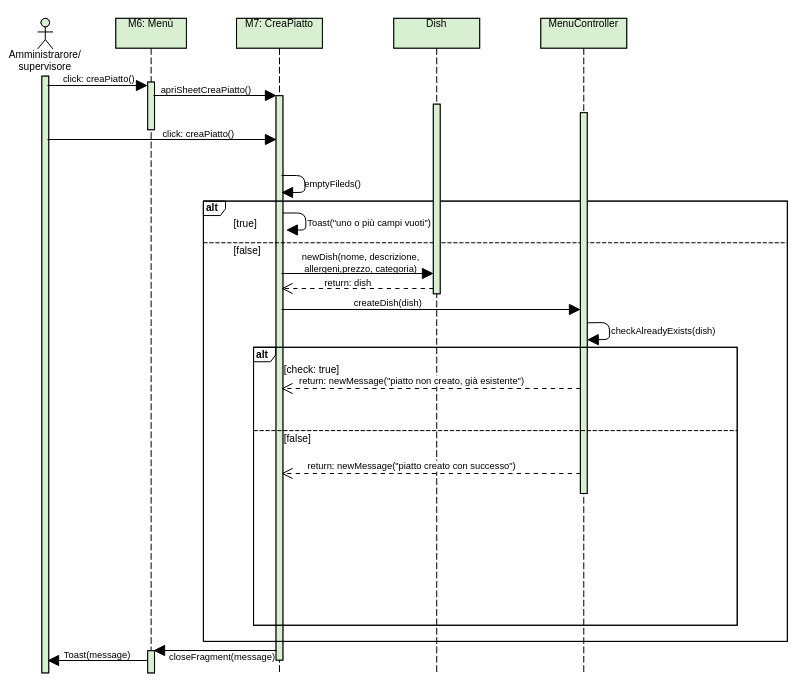
\includegraphics[scale=0.8]{img/sequence/creazionePiatto_sequence_diagram.png}
  \caption{Sequence diagram della creazione di un piatto}
\end{figure}  
\newpage
\subsubsection{Sequence diagram - Creazione notifica}
In questo \textit{sequence diagram} l'attore è un superivsore o l'amministratore, sono gli unici due ruoli con i permessi per la creazione di una. I controlli che verranno eseguiti saranno sull'esistenza della notifica, ed eventualmente se uno o più campi sono vuoti o non validi, in entrambi casi se la notifica verrà valutata "non valida", il sistema farà apparire a schermo un messaggio con scritto "errore nella creazione della notifica".
\begin{figure}[H]
  \centering
  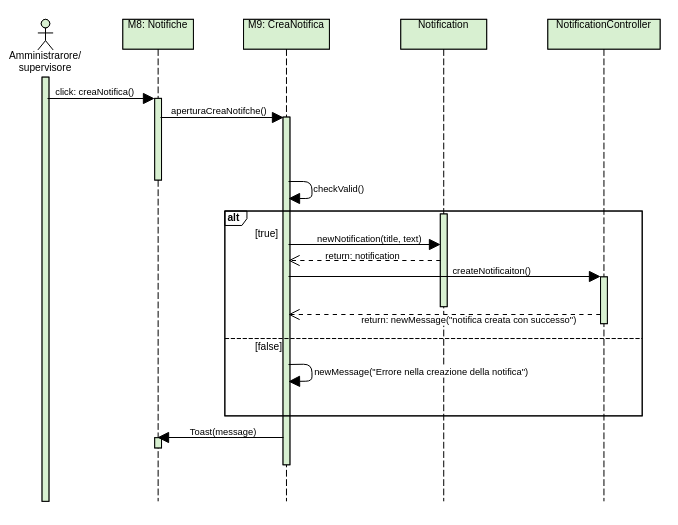
\includegraphics[scale=0.9]{img/sequence/creazioneNotifica_sequence_diagraem.png}
  \caption{Sequence diagram della creazione di una notifica}
\end{figure}  
\newpage
\subsection{State chart}
Gli \textit{state chart} sono un tipo di diagramma che descrivono il comportamento di, tramite eventi che potrebbero accadere per ciascuno stato.
Qui di seguito, analizzeremo gli \textit{state chart} dell'interfaccia grafica.
\subsubsection{State chart - Notifiche}
In questo \textit{state chart} viene analizzata l'interfaccia grafica relativa alla sezione delle notifiche (punto 13).
\begin{figure}[H]
  \centering
  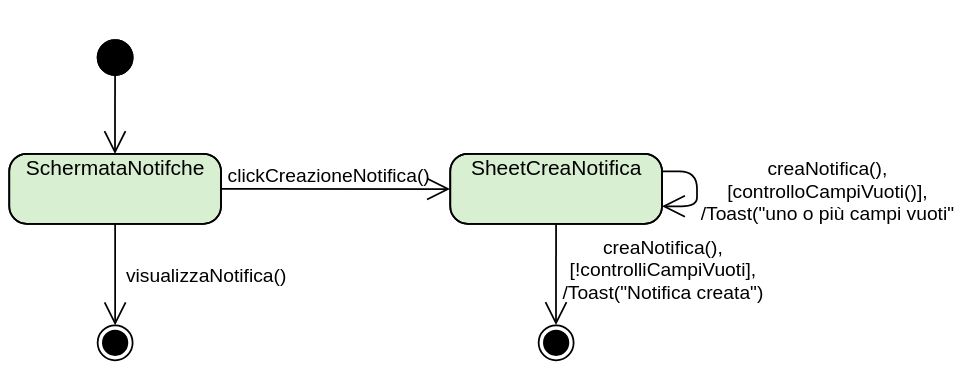
\includegraphics[scale=0.6]{img/stateChart/gestioneNotifiche_state_chart.png}
  \caption{State chart diagram della gestione delle notifiche}
\end{figure}  

\newpage
\subsubsection{State chart - Menù}
In questo \textit{state chart} analizzeremo la gestione del menù nel suo insieme, principalmente guardandolo dal lato dell'interfaccia grafica (punto 3).
\begin{figure}[H]
  \centering
  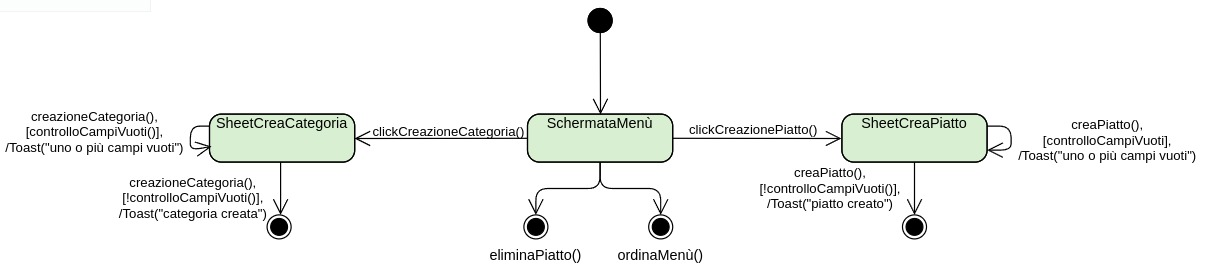
\includegraphics[scale=0.4]{img/stateChart/gestioneMenu_state_chart.png}
  \caption{State chart diagram della gestione del menù}
\end{figure}  

\newpage
\subsubsection{State chart - Tavoli}
Questo \textit{state chart}, è quello che analizzerà la gestione dei tavoli, sempre dal lato dell'interfaccia grafica (punto 6).
\begin{figure}[H]
  \centering
  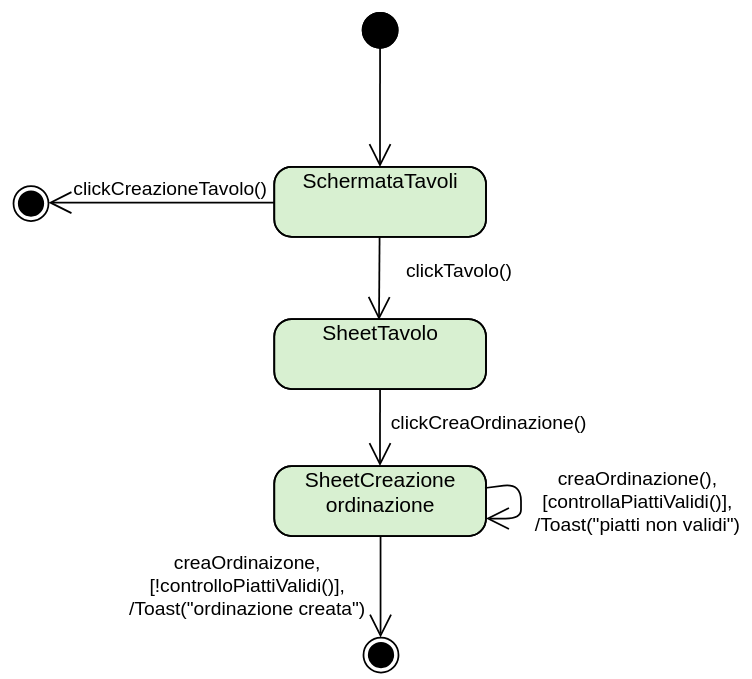
\includegraphics[scale=0.6]{img/stateChart/gestioneTavoli_state_chart.png}
  \caption{State chart diagram della gestione dei tavoli}
\end{figure}  
\newpage
\subsubsection{State chart - Login e Creazione utenza}
Per ultimo, analizzeremo la parte del login e della creazione di un utenza (punto 1).
\paragraph{Creazione utenza -} qui sotto è rappresentata la creazione di un utenza.
\begin{figure}[H]
  \centering
  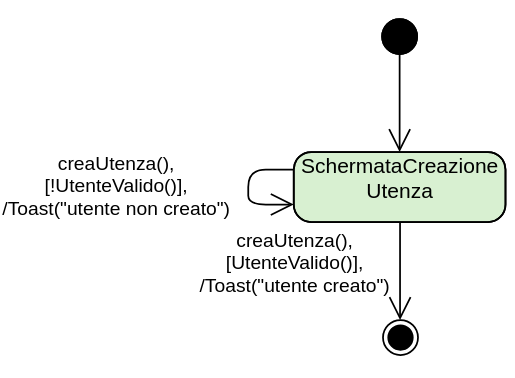
\includegraphics[scale=0.8]{img/stateChart/creazioneUtenza_state_chart.png}
  \caption{State chart diagram della creazione utenza}
\end{figure}  
\newpage
\paragraph{Login -} Qui sotto invece, è rappresentato il login (punto 1).
\begin{figure}[H]
  \centering
  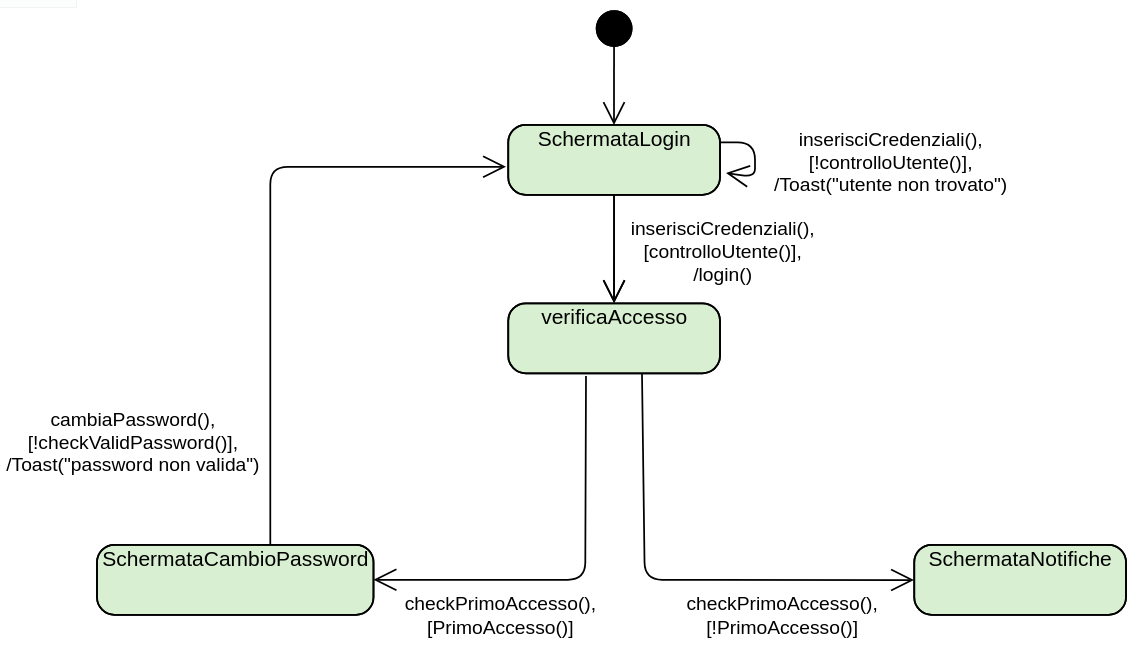
\includegraphics[scale=0.5]{img/stateChart/login_state_chart.png}
  \caption{State chart diagram del login}
\end{figure}  